\documentclass{article}
\usepackage{hyperref}
\usepackage{graphicx}
\usepackage{indentfirst}

\title{The Format-ional Edge: How I Beat Horse Racing's Keepers of The Data}
\author{Jack Karisch}
\date{June 2021}

\begin{document}

\begin{figure}
  \centering
  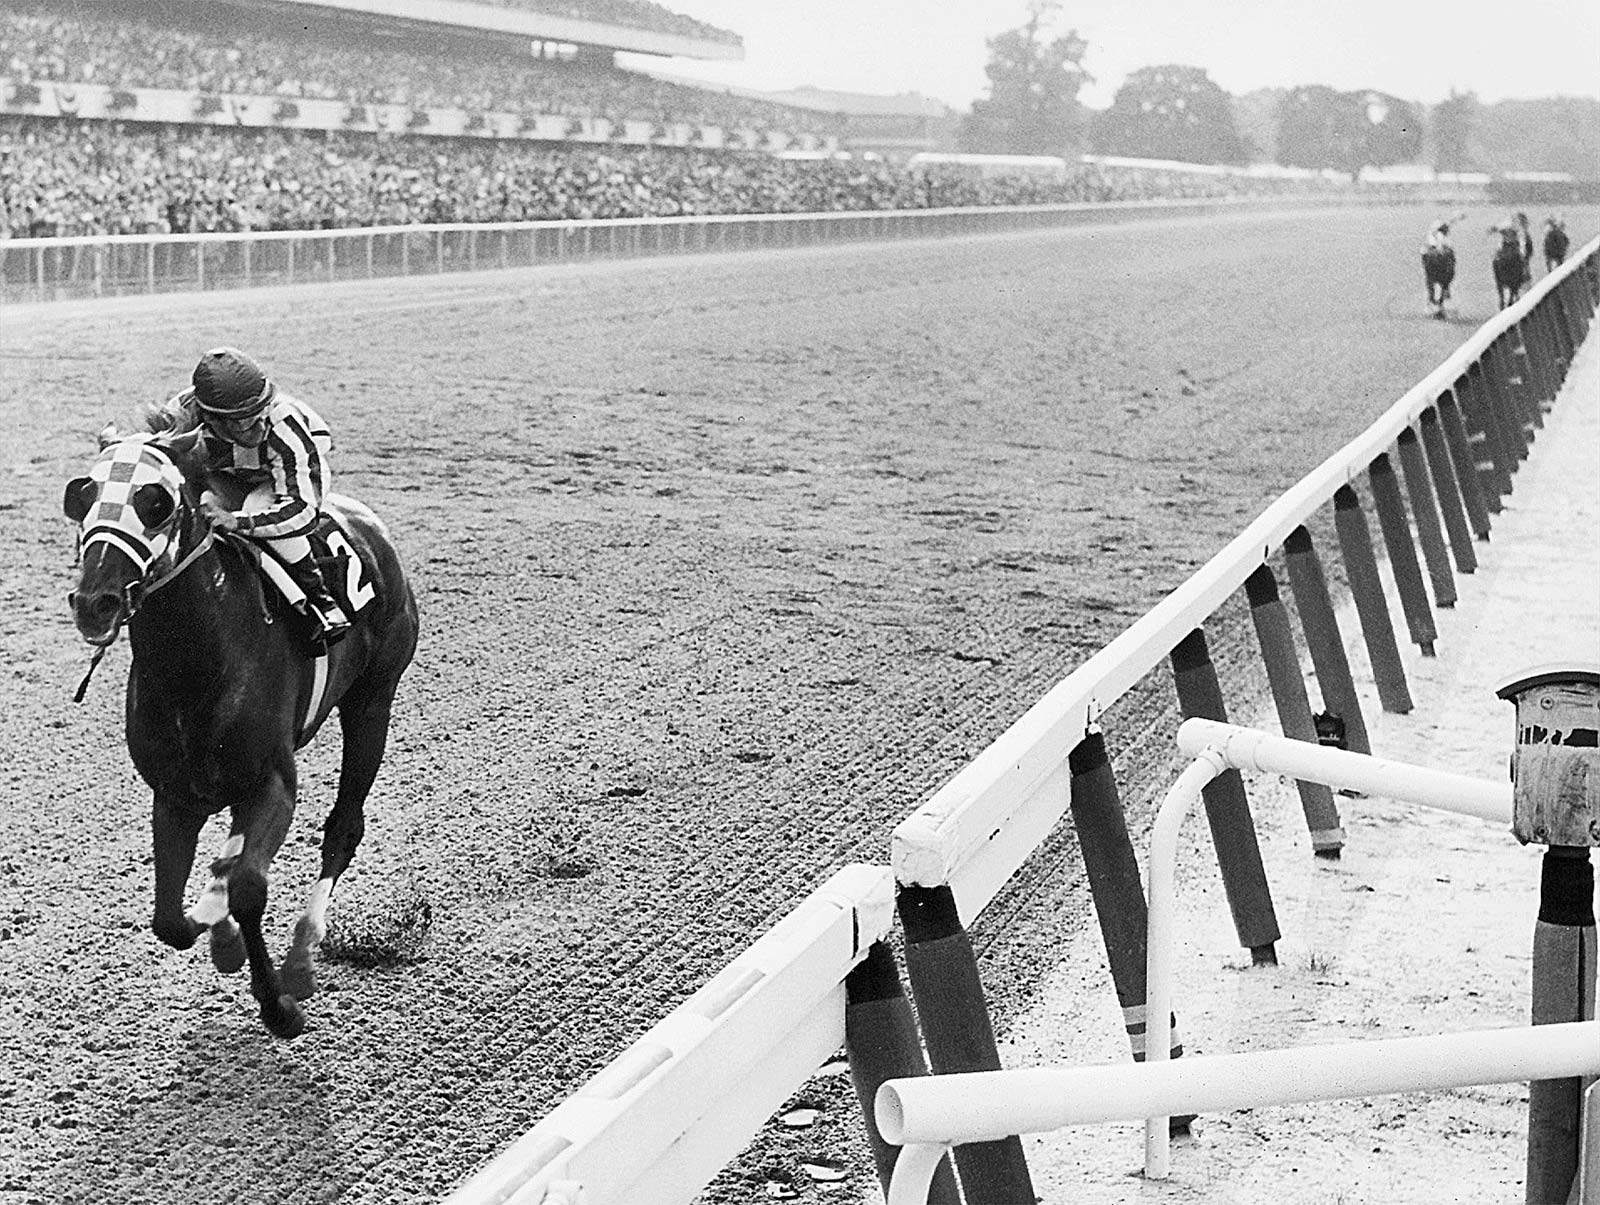
\includegraphics[width=10cm]{images/secretariat.jpg}
\end{figure}

\maketitle

\section*{\centering {Introduction}}

Horse racing has a data problem. I became aware of this problem when I attended my first races in 2016. The prior year I had read the late Bill Nack's \href{https://www.amazon.com/Secretariat-William-Nack/dp/0007410913/ref=tmm_pap_swatch_0?_encoding=UTF8&qid=1624916071&sr=8-2}{Secretiat} (which I highly recommend); this sparked an interest in horse racing that I was able to indulge after a move to New York, home to some of the most legendary tracks in the country (Belmont Park, Aqueduct, Saratoga, etc.). Notwithstanding the loss of my wallet, I had a good time at the track the first time I went, and my brother and I were hooked. We now make it a point to try to attend the Belmont Stakes every year. However, the more time I spend around horse racing the more bothered I am by the sport's broken data distribution system. 

Participating in the betting on race day necessitates the purchase of the Daily Racing Form's past performances charts for the races. As the name suggests, these sheets give horseplayers information about each horse's racing and workout performances in the months and years prior. Past performances (PPs) are the industry standard for betting information. They are not sufficient in this analytic era. Racing is one of the only sports that has enjoyed extensive freedom from regulation on betting, and has therefore had way more time than the others to figure out how it wants to handle its data and share it with bettors. PP sheets as data transfer tool were acceptable through the 80s, maybe even up to the early 2000s. Gamblers didn't have the resources or skills required to process and analyze the data, and there were no competing sports outperforming racing on the data front. This is no longer the case.

I recently happened across a \href{https://www.youtube.com/watch?v=4B0mGYZqElo}{video} from Bloomberg Quicktake that documents the career of Bill Benter. In the early 2000s, Benter, a blackjack player frustrated by casinos' attempts to eradicate card counting, sought another game with better earnings potential. A friend and fellow gambler recommended horse racing, and together they decided to turn their attention to the turf. By hand, they laboriously entered the results from a great number of races into a database, a process that took them nine months. Once they had a large cache of results, they started mining it for exploitable patterns that would be invisible to the average bettor, earning millions along the way. To me, the most interesting part of the endeavor is that Benter, an American gambler, focused his efforts exclusively on the Hong Kong racing scene. Unsurprisingly, the reason he did this is because the Hong Kong jockey club maintained more fulsome and useful information than the American, and also because the horses raced more frequently, increasing the amount of data on each, and at far fewer tracks, limiting variability. The American Jockey Club was effectively out-competed on the basis of its subpar data by its Chinese coutnerpart for Benter's interest and (more importantly) his money.

Since this was all happening in the early 2000s, it's reasonable to ask what The Jockey Club (the governing body of American racing) has done in the intervening years to rectify the issue. They have taken steps to do so. The official record-keeping wing of The Jockey Club and the Thoroughbred Racing Associations, Equibase, supplies information on entries, horses and selections. It also offers PPs for a nominal fee. Notably, the results for practically every race run since 1991 can be accessed in PDF form, and this year marks the first that the \href{http://jockeyclub.com/factbook/ARM/2021_arm.pdf}{American Racing Manual}, a massive almanac of historical and current racing stats, is available free of charge, also in PDF form. However, Equibase has stubbornly refused to release raw data to the public. The Thoroughbred Idea Foundation, a think tank whose mission is to improve the sport of racing to drive general interest and gambling participation, released a \href{https://racingthinktank.com/application/files/5015/5231/3157/20190311_-_TIF_REPORTS_-_Embracing_a_Future_with_Free_Racing_Data.pdf}{report} in 2019 that perfectly outlines the issue. The report lays out the case for more comprehensive data in useful formats distributed at low/no cost. It takes the view that ``[t]he current cost of racing data, and the inflexible formats in which it is provided, serve as hurricane-force headwinds in today’s wagering environment", especially given the rapid increase in public interest in gambling on conventional sports and the corresponding favorable legislative response, as well as the willingness of major sports leagues to provide fairly comprehensive stats free of charge (I would particularly like to single out the MLB here, which releases an astonishing amount of data in real time for free through a well-maintained API).

As a fan of horse racing and a statistics major, I have been interested in the issue of horse racing data for some time. Faced with the glacial pace of Equibase's acquiescence to the data revolution, some time last year I began to explore the possibility of scraping what data I could from Equibase's site and throwing it into a CSV for basic analysis. Over time my aspirations expanded, until I made it my goal to pull a huge quantity of race results (say several years) as PDFs and parse them into as much usable data as possible. It was a rocky road, with many obstacles, but for every problem I encountered I was able to find a workaround, some more elegant than others. I have succeeded in pulling five years of results from Equibase, parsing the data and placing it into a SQL database. To give an idea of the scale of this data, the horse table has more than two million entries, each corresponding to a single race performance by a single horse. It's not perfect, but I estimate that more than 99\% of the data is accurate.

My database has given me an edge over most horseplayers; not an informational edge, since everything in the database is available for free to anyone with an internet connection, but an advantage in format (a ``format-ional" edge, if you will), allowing me to turn loose a vast amount more processing power than the average bettor on the available data.

This writeup documents how I beat the overzealous guardians of horse racing data (as I came to think of Equibase throughout the process). I present two different versions: one simple and one technical. Casual readers will prefer the simple version, but anyone wanting to do what I've done or apply my methods to a similar webscraping problem will want to read the technical version.

\section*{\centering {The Simple Version}}

\noindent These are the main issues I faced during the process:
\begin{enumerate}
  \item Equibase is evil (I'm only mostly kidding)
  \item PDFs are frustrating (anyone who has tried to copy/paste a large amount of text from a complex PDF can attest to this)
  \item Horses don't cooperate (why can't they just always finish races?)
\end{enumerate}

\noindent I will describe below the nature of these issues and how I overcame each one.

\subsection*{\centering 1. Equibase Is Evil}

Equibase has done a great deal of good for the sport of racing (not to mention this entire project would have been DOA if they didn't provide results PDFs in the first place), so my calling them evil is more an indication of the amount of frustration they have caused me than a legitimate accusation. Setting aside my displeasure at their continued refusal to just release their data to the public, my frustration at Equibase can be summed up in a single hideous word: Incapsula.

Incapsula, as I came to understand, is a third-party bot detector whose sole responsibility is to prevent people from doing exactly what I have done with this project. Basically, when you click a link or type in a URL on your browser, you send a request to a server that sends back the page/video/information you asked for. Computers can do this as well; it's very easy to send a request from within Python. However, requests originating from different sources have different signatures, and Incapsula leverages these signatures to identify requests coming from a computer and block the requested information from going out. There are multiple reasons a site might want to do this. The most obvious is that serving requests costs money and bots can send orders of magnitude more requests than people. In Equibase's case, I suspect they keep Incapsula around so that computationally adventurous horseplayers can't pull down huge numbers of PDFs quickly and easily, circumventing the need to pay for data. More sophisticated (i.e. nerdier) people than I can defeat these bots directly by spoofing their signatures, but it's beyond my abilities.

I had to get creative. I relied on two key oversights by Equibase: their site URLs are uniformly generated, and they list every track that held racing on a particular date. Some sites assign URLs randomly. Picture a YouTube video URL. The first part is obviously always the same (``www.youtube.com/") but the next part gets more interesting (``watch?v=4B0mGYZqElo"). This is a random string of letters and numbers that makes it basically impossible to brute force a search of all YouTube videos (to be clear, I don't think that's why YouTube did this, but the effect is independent of the reason). In contrast, Equibase uses consistent URLs for its pages, e.g. ``?mo=5\&da=14 \&yr=2021\&trackco=ALL". Careful study of this link will reveal that it points to a page that shows all tracks that held races on May 14, 2021. This is an exploitable pattern. I was able to generate URLs for any given date (I just batch-generated 365 at a time by picking a particular year), then pull the HTML returned by these links onto my computer. I searched through these HTML files (not literally, I used Python) and pulled out links to the results pages of every track that held racing on that day. Then all I had to do was visit those links and download the PDFs they returned.

I automated the downloading part of the process in two ways. For the HTML, I used a program called AutoHotKey to create a script that repeatedly entered keystrokes as if I were typing them myself. I would batch open say 50 date tabs, then start AutoHotKey, which would control-s (save webpage as HTML) then control-w (close tab) 50 times. For the PDFs, I set my browser to auto-download any PDFs I loaded from the web. Then all I had to do was batch open a huge number of PDFs (usually 100) and they would all download within 10 seconds. Every once in a while Equibase would seem to notice that I was gaming the system and it would toss me an ``Are you a bot?" captcha test, which slowed me down a bit. This is obviously still a fairly labor-intensive process, but I estimate that I can pull somewhere around 5000 results PDFs per hour using it.

\subsection*{\centering 2. PDFs Are Frustrating}

Solving the first problem left me with a large number of PDFs on my hard drive and not much else. I had to figure out a way to get my computer to read those PDFs. This is surprisingly hard to do. Regular text documents store text as bits, which are easily understood by a computer. Basically, man and computer read them the same way, but the computer does it in binary. PDFs store text by location on the page (e.g. put a ``J" at coordinate (x, y)), which is very hard for a computer to understand. It took me a couple of days of searching to come up with a solution. 

There is a Postscript (the language PDFs are written in) interpreter called Ghostscript that can process PDF files. It reads the text letter-by-letter then tries to recreate the PDF as a regular text file based on the coordinate of each letter. It renders individual files fairly accurately, but it struggles with consistency across a large batch of similar files, which is of paramount importance for heavy text parsing. To improve consistency, instead of converting the PDFs directly to text files, I first converted them to XML format. Basically, I converted them into a similar format to the one the computer uses to render PDF documents. This format is terrible for humans, but great for computers. I wrote a program that reads each letter and its location in the PDF from the XML file, then assigns it a particular spot in a particular line based on some rules I defined through trial and error. This hacked together parser turned out to be extremely consistent, although it separates all text in a line by no more than one space, making it somewhat difficult for humans to read.

\subsection*{\centering 3. Horses Don't Cooperate}

I was getting close, or so I thought. I now had a folder full of text files that my computer could understand. I got to work writing a program to iterate through these files and extract information from the lines based on a set of rules. These rules were pretty simple and assumption-heavy, so my program was prone to failure. It would process a few files, then hit a snag (e.g. the jockey's name had a hyphen in it, and my program expected only letters). I would generalize the program to capture the new pattern then try again, and hit another snag. Over time, I was sacrificing robustness and interpretability in my program for generalization. In order to parse as much information as possible, I needed to make my program just general enough to capture the edge cases, but not so general that it would capture too much. I basically had to account for every crazy event that can happen in horse racing. Dead heat? Broken algorithm. Fog obscuring the track, meaning the split times were left blank? Broken algorithm. I found myself getting upset with horses for not finishing races, since I had to adjust the total number of horses running at each point of call of the race. I fixed that issue and was feeling pretty good about myself then ran into a horse that didn't even leave the gate. This turned out to be the perfect storm of bad luck, breaking my program's search function across multiple lines and taking me hours to fix. 

This part of the process turned into a battle of attrition, and I kept plugging away a few hours every day. Over time, my program would run longer and longer before hitting anomalies, until I could parse an entire year of race results (over 5,000 PDFs, containing more than 40,000 races) without any errors. This is the kind of mind-numbing work that's required with a project like this, and I believe Equibase is counting on most people giving up before they get through it. I almost did a few times, but I kept coming back until I had prevailed.

\bigbreak

The final piece was moving all this parsed data into a PostgreSQL database. This is not difficult, and despite a few hiccups didn't take me very long. I had finally beaten Equibase.

\section*{\centering {The Technical Version}}

This account of the process will be more technical and less interesting than the prior one, but I want to document more specifically how I went about solving this problem, both for others that may want to do something similar, and for myself so I can remember how it all works. It's helpful to have read the simple version before reading this one. As above, I'll break it into three parts:

\begin{enumerate}
  \item Obtaining the PDFs
  \item Converting the PDFs
  \item Parsing the TXTs
\end{enumerate}

\noindent I make an effort to link to relevant files on GitHub when they are discussed to make it easy to follow along.

\subsection*{\centering 1. Obtaining the PDFs}

To work around Equibase's bot detector, I had to personally manage any requests to Equibase as a human (I use the term "personally manage" very liberally here, as we will see), then offload any processing of the information returned by these requests to the computer.

The first step was to figure out how to find the races on the Equibase site. I leveraged the fact that Equibase's search page allows users to enter a date, then displays every track that had racing on that date. The URLs to access these date pages are very regular (think day=x\&month=y), so I threw together an \href{https://github.com/Real-Karisch/horseData/blob/master/excel/generateDayLinks.xlsx}{excel file} that can generate links for every day in a given year.

Now comes a part where I needed to use my humanity to interact with the Equibase site. To save time, I found a \href{https://www.openmultipleurl.com/}{website} that will open up to 250 browser tabs if provided with links. I went in batches of 50 for this step, copying links from my excel file, then dropping them into the website. In order to get the links for each track on each day, I needed to parse the HTML of the pages. To do this, I needed to download the HTML version of the pages to my computer so Python could access them. I turned to AutoHotKey to automate this part of the process. I created an \href{https://github.com/Real-Karisch/horseData/blob/master/python/convertPDF/webScrape/saveHtmlHotkey.ahk}{AHK script} that presses control-s (save), "equibase[i]" (name file), control-w (close tab) for an iterator i 50 times. The iterator is necessary to avoid name conflicts in the download folder. I then used a \href{https://github.com/Real-Karisch/horseData/blob/master/python/convertPDF/webScrape/htmlMgmt.py}{Python script} to rename the files in the folder to make way for the next batch.

Once I had the HTML files downloaded, I used a \href{https://github.com/Real-Karisch/horseData/blob/master/python/convertPDF/webScrape/saveTrackUrlsFromFiles.py}{Python program} to search through them and pull out the track day URLs from each. This required a bit of manipulation since the URLs in the HTML files don't lead directly to the PDFs, but it was easy enough to modify. This program outputs a CSV file containing the URLs.

Now that I had the URLs, all I needed to do was, once again leveraging my personhood, go back to the OpenMultipleURL site and start feeding them in. This step required some additional setup for maximum efficiency, however. First, I set the browser to auto-download every PDF file it loads. Then, I made sure the ``Ask me before downloading things" option is set to ``No". I started dropping the URLs in and downloading en masse. I found batch sizes of 100 worked well, but I experimented successfully with sizes up to 250. Every once in a while, I got captchas (generally a bunch all at once) asking to verify that I was human. I would fill one out, then close any other captcha tabs and re-run them and it generally wouldn't bother me again.

\subsection*{\centering 2. Converting the PDFs}

This part of the process is relatively straightforward. I used Ghostscript to convert the PDFs to text. I found that the straight conversion had too little consistency, so I converted to XML first then to TXT. To convert to XML, I wrote an extremely simple \href{https://github.com/Real-Karisch/horseData/blob/master/python/convertPDF/webScrape/pdf2xml.py}{script} that iterates through a folder, converting each file and putting the result in a different folder.

The next step was similarly straightforward, although somewhat more labor-intensive. I found consistent patterns in the placement of the lines in the PDFs (e.g. the lengths in a running line result are size 6 font, offset vertically by a consistent amount from the size 8 font place records). Through trial and error, I wrote a \href{https://github.com/Real-Karisch/horseData/blob/master/python/convertPDF/webScrape/xml2txt.py}{program} that looks at each letter and determines which line it should inhabit (y coordinate) and which position in that line it should inhabit (x coordinate) in the final text document based on its location in the PDF. To illustrate, here is the word "January" from a PDF as rendered by the XML parser:
\bigbreak

\ttfamily
<span bbox="95 32 125 32" font="Helvetica-Bold" size="8.0000">\par
<char bbox="95 32 99 32" c="J"/>\par
<char bbox="99 32 104 32" c="a"/>\par
<char bbox="104 32 108 32" c="n"/>\par
<char bbox="108 32 113 32" c="u"/>\par
<char bbox="113 32 118 32" c="a"/>\par
<char bbox="118 32 121 32" c="r"/>\par
<char bbox="121 32 125 32" c="y"/>\par
</span>
\bigbreak

\rmfamily

\noindent The parser sees that all these letters have the same vertical coordinate in the PDF (32) and consecutive horizontal coordinates spanning 95 - 125, and places them on a single line all adjacent to one another.

My program places single spaces between both large and small horizontal positional gaps in the PDF, making it very difficult for humans to read. Here is an example next to the corresponding PDF text:

\begin{figure}[h]
  \centering
  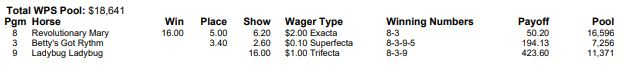
\includegraphics[width=12cm]{images/betLinesPDF.JPG}
\end{figure}

\ttfamily
\noindent Total WPS Pool: \$18,641\par
\noindent Pgm Horse Win Place Show Wager Type Winning Numbers Payoff Pool\par
\noindent 8 Revolutionary Mary 16.00 5.00 6.20 \$2.00 Exacta 8-3 50.20 16,596\par
\noindent 3 Betty's Got Rythm 3.40 2.60 \$0.10 Superfecta 8-3-9-5 194.13 7,256\par
\noindent 9 Ladybug Ladybug 16.00 \$1.00 Trifecta 8-3-9 423.60 11,371\par
\bigbreak

\rmfamily


\subsection*{\centering 3. Parsing the TXTs}

It will surprise no one that I leaned extremely heavily on regular expressions for the final part of the process. This is a cut and dried text pattern matching exercise. For reference, practically all of the regular expressions I used for text parsing can be found in \href{https://github.com/Real-Karisch/horseData/blob/master/python/convertPDF/infoFns/regexPatterns.py}{this file}. Each one is exactly as general as it needs to be and no more. To parse text files, I use a \href{https://github.com/Real-Karisch/horseData/blob/master/python/convertPDF/driver.py}{script} to drive the process, scanning each file and splitting it up into individual races, then sending those races to a child function that divides them further into segments based on the type of information (general race, horses, timing, betting, runningnline, trainers/owners). These sections are then sent to \href{https://github.com/Real-Karisch/horseData/tree/master/python/convertPDF/infoFns}{corresponding functions} for parsing. 

The parsing functions identify which line is which, then apply regular expressions correspondingly. The regular expressions match the line, then subgroups are parsed further or stored in dictionaries as strings to be placed into a database. The lines follow set patterns which are generally easy to parse, but some small amount (less than 5\%) will deviate from the pattern, and require tweaks to the regular expressions to catch them. Often this just means adding a letter or symbol to a capture group, but it can necessitate a full overhaul of the expression. Here is an example of a line in the text document next to the regular expression that matches it:
\bigbreak

\ttfamily
\noindent 3 Betty's Got Rythm 3.40 2.60 \$0.10 Superfecta 8-3-9-5 194.13 7,256
\bigbreak

\noindent `\^{} \textbackslash d?\textbackslash d[ABCXabcx]? [\^{}0-9]+ (\textbackslash d?\textbackslash d?\textbackslash d.\textbackslash d\textbackslash d) (\textbackslash d?\textbackslash d?\textbackslash d.\textbackslash d\textbackslash d)()(.*)\$'

\bigbreak

\rmfamily

`\texttt{\^{} \textbackslash d?\textbackslash d[ABCXabcx]?}' matches the horse program number (3), `\texttt{[\^{}0-9]+}' matches the horse name (Betty's Got Rythm), two `\texttt{(\textbackslash d?\textbackslash d?\textbackslash d.\textbackslash d\textbackslash d)}' groups match the place (3.40) and show (2.60) payouts, and `\texttt{(.*)\$}' matches the rest of the line (\$0.10 Superfecta...). The last group gets sent to another regular expression for further parsing.

The last step is to take the parsed data and populate a SQL database. This is very similar to a \href{https://github.com/Real-Karisch/baseballData}{project} I worked on in which I created a database of MLB stats, so it was old hat for me. I created a \href{https://github.com/Real-Karisch/horseData/blob/master/python/populateDB.py}{script} with a function that runs the parser on all the files in the set, then hands the parsed data off to a function that puts it into two PostgreSQL tables (``horses" and ``races"). The ``races'' table contains data on each race in the database (e.g. post time, weather and track conditions, betting information, etc.), and the ``horses'' table contains entries for every horse that ran in these races. Every line in the ``horses" table is related to exactly one line in the ``races'' table, but multiple lines in the ``horses'' table will be related to the same race. The code for creating this database can be found \href{https://github.com/Real-Karisch/horseData/blob/master/sql/horses.sql}{here}.


\end{document}